\documentclass[border=2pt]{standalone}

\usepackage{tikz}

\begin{document}
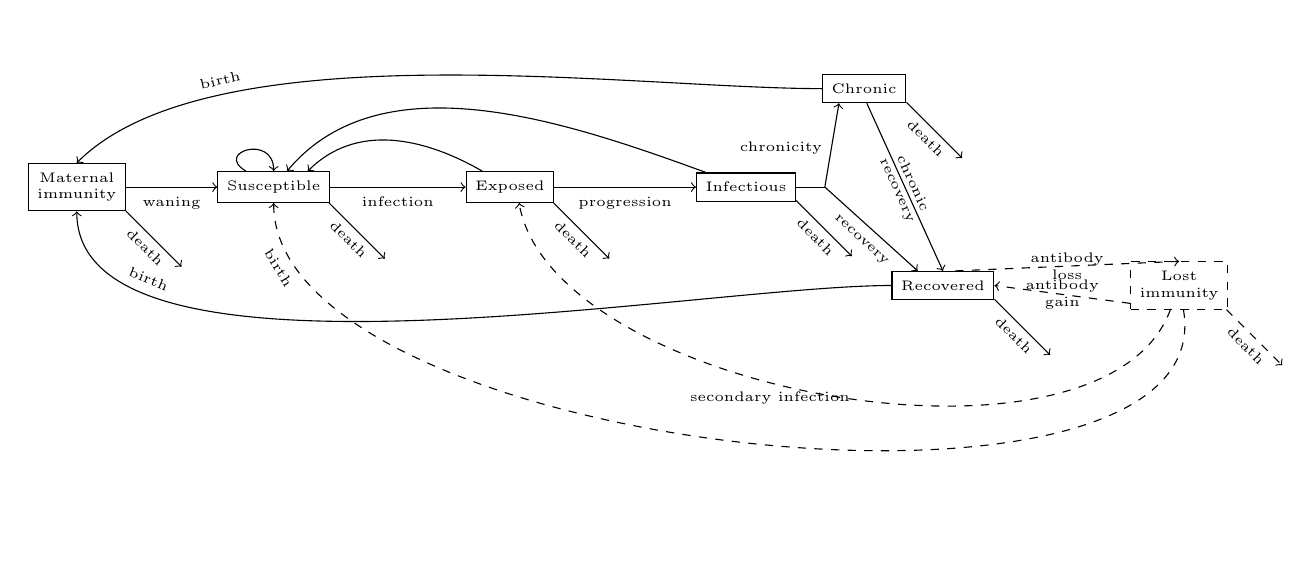
\begin{tikzpicture}[compartment/.style = {rectangle, draw}, font=\fontsize{5pt}{6}\selectfont]
  % Compartments.
  \node at (0, 0) [compartment, align=center, name=MaternalImmunity] {Maternal\\immunity};
  \node at (2.5, 0) [compartment, name=Susceptible] {Susceptible};
  \node at (5.5, 0) [compartment, name=Exposed] {Exposed};
  \node at (8.5, 0) [compartment, name=Infectious] {Infectious};
  \node at (10., 1.25) [compartment, name=Chronic] {Chronic};
  \node at (11., -1.25) [compartment, name=Recovered] {Recovered};
  \node at (14, -1.25) [compartment, align=center, dashed, name=Partial] {Lost\\immunity};

  % Location for branch from Infectious to Chronic and Recovered.
  \coordinate (recovery) at (9.5,0);

  % Infection-related processes.
  \draw [->] (MaternalImmunity)
             to node [below] {waning}
             (Susceptible);
  \draw [->] (Susceptible)
             to node [below] {infection}
             (Exposed);
  \draw [->] (Exposed)
             to node [below] {progression}
             (Infectious);
  \draw [  ] (Infectious)
             to node [] {}
             (recovery);
  \draw [->] (recovery)
             to node [left, yshift=-1pt] {chronicity}
             (Chronic.210);
  \draw [->] (recovery)
             to node [sloped,below,yshift=-0.5pt] {recovery}
             (Recovered.150);
  \draw [->] (Chronic.280)
             to node [sloped, align=center] {chronic\\recovery}
             (Recovered.90);
  \draw [->, dashed] (Recovered.50)
             to node [out=80, in=45, looseness=0.6,align=center] {antibody\\loss}
             (Partial.90);
  \draw [->, dashed] (Partial.200)
             to node [out=200, in=350, looseness=0.6,align=center] {antibody\\gain}
             (Recovered.0);
  \draw [->, dashed] (Partial.250)
             to [out=250, in=280, looseness=0.75] node [below, pos=0.57] {secondary infection}
             (Exposed.300);

  % Births
  \draw [->] (Susceptible.150)
             to [out=150, in=90, looseness=3.5] node [] {}
             (Susceptible.90);
  \draw [->] (Exposed.150)
             to [out=150, in=45] node [] {}
             (Susceptible.25);
  \draw [->] (Infectious.160)
             to [out=160, in=50, looseness=0.9] node [sloped, above, pos=0.85] {}
             (Susceptible.50);
  \draw [->] (Chronic.180)
             to [out=180, in=45, looseness=0.65] node [sloped, above, pos=0.75] {birth}
             (MaternalImmunity.90);
  \draw [->] (Recovered.180)
             to [out=180, in=270, looseness=0.6] node [sloped, above, pos=0.8] {birth}
             (MaternalImmunity.270);
  \draw [->, dashed] (Partial.280)
             to [out=280, in=270, looseness=0.7] node [sloped, below, pos=0.92] {birth}
             (Susceptible.270);

  % Deaths
  \draw [->] (MaternalImmunity.334)
             to node [sloped, below, yshift=1pt] {death}
             +(315: 1);
  \draw [->] (Susceptible.344)
             to node [sloped, below, yshift=1pt] {death}
             +(315: 1);
  \draw [->] (Exposed.340)
             to node [sloped, below, yshift=1pt] {death}
             +(315: 1);
  \draw [->] (Infectious.345)
             to node [sloped, below, yshift=1pt] {death}
             +(315: 1);
  \draw [->] (Chronic.342)
             to node [sloped, below, yshift=1pt] {death}
             +(315: 1);
  \draw [->] (Recovered.345)
             to node [sloped, below, yshift=1pt] {death}
             +(315: 1);
  \draw [->, dashed] (Partial.333)
             to node [sloped, below, yshift=1pt] {death}
             +(315: 1);
\end{tikzpicture}


\end{document}
